\documentclass[a4paper, 12pt, openany]{book} %chose the paper size and font size. Openany ensures that all all chapters and similar may begin at any page, not only odd pages. For the introductory pages and appendices we want openany, but for chapter pages in the main content we want chapters to begin only on odd pages (right hand side). The book class ensures that the margins are automatically adjusted such that left hand pages are slightly moved to the left and vice versa at the right, which makes the thesis very readable and good looking when printed in bound book format.
\usepackage[utf8]{inputenc} %to manage special characters
\usepackage[T1]{fontenc} %to manage special characters
\usepackage[Bjarne]{fncychap} %fancy chapter style (many more available, like Sonny or Lenny etc.)
\usepackage{fancyhdr} %to customize the headers
\usepackage[lmargin=1.5in, rmargin=1in, tmargin=1in, bmargin=1in]{geometry} %sets the margins for the pages
\setcounter{tocdepth}{2} %table of contents number depth for subsections (2 = x.x.x)
\setcounter{secnumdepth}{4} %numbering depth for headers for subsections in the text(4 = x.x.x.x)
\usepackage{url} %to include urls
\usepackage{listings} %include this if you want to include code in the thesis
\usepackage{amsmath,amssymb} %mathematical package
\usepackage{siunitx} %includes SI-units
\usepackage[bf]{caption} %makes float captions bold
\usepackage{array, booktabs} %to make better tables
\usepackage{graphicx} %to include graphics
\usepackage{float} %to include floats
\usepackage[export]{adjustbox} %to adjust floats
\usepackage{subfig} %to include subfigures
\usepackage{chngcntr} %will make it possible to change the counter for tables, figures etc. such as below
\counterwithin{figure}{section} %change counter for figures within sections (also possible to choose for each chapter
\counterwithin{table}{section} %change counter for tables within sections
\usepackage{color, xcolor} %edit e.g. text colors

\usepackage[backend = biber,
            style = numeric,
            date = long,     % Long: 24th Mar. 1997 | Short: 24/03/1997
            sorting = none,
            maxcitenames = 3,   % max names to include before et. al.
            ]{biblatex} %customize the look of your citations and bibliography
\addbibresource{bibliography.bib} %declare the bibliography resource
\usepackage{comment} %to be able to comment out sections in the .tex files
\usepackage{afterpage} %to customize page commands such as below
\newcommand\myemptypage{
    \null
    \thispagestyle{empty}
    \addtocounter{page}{-1}
    \newpage
    } %sets new page command to insert an empty page without adding to the page counter or having a page number




\begin{document}
%%%%%%%%%%%%%%%%%%%%%%%%%%%%%%%%%%%%%%%%%%%%%%%%%%%%%%%%
%\begin{comment}
% The title page:
% For NTNU students this page will be generated automatically when submitting your paper, and should not be included in the final file from Latex. Delete or comment out the title page setup. The final report should then start with the first page being the abstract. I have included a title page here so it is possible to see how it may look like, and for those who does not get an automatically generated title page. Of course you will need to change the names and titles etc. to your case.

%the title page should be an odd page (right hand side)

\begin{titlepage}
\newgeometry{left=1.6in, right=2in}
\vspace*{1.5cm}

\noindent  \textcolor{gray}{\large Nina Salvesen} \\
\vspace{1cm}

\noindent \textbf{\Large The title of your master's thesis should be written here} \\
\vspace{0.5cm}

\noindent {\large Any undertitle is written here} \\



\vspace{7cm}
\noindent Master's thesis in Physics and Mathematics \\
Supervisor: Supervisor Name \\
Co-supervisor: Co-supervisor Name \\
June 2022 \\

\vspace{0.2cm}
\noindent Norwegian University of Science and Technology \\
Faculty of Natural Sciences \\
Department of Physics \\

\begin{figure}[h]
    
\includegraphics[width=0.28\textwidth]{Figures/ntnu_basic.png}
\end{figure}
\end{titlepage}
\restoregeometry
\myemptypage %empty page such that the abstract starts at the first right hand side after the title page
%\end{comment}
%%%%%%%%%%%%%%%%%%%%%%%%%%%%%%%%%%%%%%%%%%%%%%%%%%%%%%%%

% The pre-chapters
\chapter*{Abstract} %pre-chapters should not be numbered, hence the "*"
\pagenumbering{roman} %introductory pages should be roman
\setcounter{page}{1}
\addcontentsline{toc}{chapter}{\protect\numberline{}Abstract} %add the chapter to the table of contents, this is not automatically added when creating unnumbered chapters (*). Add it in a chapter style, and keep all chapters on the same numberline indent regardless of number or not on the chapter
Holographic duality has been very successful at studying strongly-coupled gauge theories by mapping the problem to one of classical gravity. It is interesting to ask whether (and what) one can learn about quantum gravity by studying gauge theories in certain approximations. 

In this dissertation, we present a summary of results in the study of the BFSS matrix model at high energies or, equivalently, weak coupling, where the dual gravity picture is highly stringy. The bosonic sector is analyzed through classical, real-time numerical simulations for a range of values of $N$ (the size of matrices). We find sensitivity to initial conditions of a particular nature that suggests the following picture: typical (random) classical states of matrix theory mimic microstates of the dual gravitational theory. 

Another feature reminiscent of black hole physics is random matrix behavior. The long-time distribution of matrices evolving through classical BFSS equations of motion is shown to resemble a traceless Gaussian Unitary Ensemble (GUE). We carefully match parameters on both sides (the matrix size $N$, the energy $E$ of the state considered, and a scale parameter $\alpha$ of GUE). Lastly, we present evidence suggesting higher-order correlations than those arising from simple random matrix ensembles. We discuss possible causes and fixes. %insert the chapter text from the files

\chapter*{Preface}
\addcontentsline{toc}{chapter}{\protect\numberline{}Preface} 

Write the preface of your thesis here. \\

\noindent You may include acknowledgements and thanks as part of your preface on this page, or you may add it as a new chapter after the preface.

\tableofcontents
\addcontentsline{toc}{chapter}{\protect\numberline{}Contents}

%add to table of contents list of figures and tables, and insert list of figures and tables
\addcontentsline{toc}{chapter}{\protect\numberline{}\listfigurename}
\listoffigures
\addcontentsline{toc}{chapter}{\protect\numberline{}\listtablename}
\listoftables


\chapter*{Abbreviations}
\addcontentsline{toc}{chapter}{\protect\numberline{}Abbreviations}
% Put in your abbreviations here

List of all abbreviations in alphabetic order:

\begin{itemize}
    \item \textbf{EDA} Exploratory Data Analysis
    \item \textbf{GNNS} Global Navigation Satellite System
    \item \textbf{Mamsl} meter above mean sea level
    \item \textbf{NTNU} Norwegian University of Science and Technology
    \item \textbf{PCA} Principal Component Analysis
    
\end{itemize}
\newpage
\myemptypage
%add an empty non-counted page by the command below in order to get the first chapter on the left hand side, if needed (check your page number so that the first chapter is on an odd page)


%%%%%%%%%%%%%%%%%%%%%%%%%%%%%%%%%%%%%%%%%%%%%%%%%%%%%%%%
%Customize the layout of the main content of your thesis

\pagestyle{fancy} %set customized page style for header
\fancyhf{} %clear header and footer fields
\renewcommand{\headrulewidth}{0pt} %set to no rule
\fancyhead[LE, RO]{\thepage} %set the page number at left for even, right for odd pages
\fancyhead[RE, LO]{\leftmark} %set the chapter name at right for even, left for odd pages
%is is possible to design the header with the chapter as you wish, e.q. only the chapter or only the name, all lowercase instead etc.
%you could also design the footer if you wish, for example:
%\fancyfoot[LE, RO]{\thepage}
\setlength{\headheight}{14.49998pt} %set the header height


%%%%%%%%%%%%%%%%%%%%%%%%%%%%%%%%%%%%%%%%%%%%%%%%%%%%%%%%
%main content 

\pagenumbering{arabic}
\chapter{Introduction}

% The subsections written are only suggestions, to display how sections and subsections may look for your thesis

Black Holes are notorious for seemingly violating sacred laws of physics. Perhaps the most significant is the quantum mechanical principle of reversibility: Black holes radiate and destroy information through Hawking radiation. Attempts to 

Lorem ipsum dolor sit amet, consectetur adipiscing elit, sed do eiusmod tempor incididunt ut labore et dolore magna aliqua. Ut enim ad minim veniam, quis nostrud exercitation ullamco laboris nisi ut aliquip ex ea commodo consequat. Duis aute irure dolor in reprehenderit in voluptate velit esse cillum dolore eu fugiat nulla pariatur. Excepteur sint occaecat cupidatat non proident, sunt in culpa qui officia deserunt mollit anim id est laborum.

Sed ut perspiciatis unde omnis iste natus error sit voluptatem accusantium doloremque laudantium, totam rem aperiam, eaque ipsa quae ab illo inventore veritatis et quasi architecto beatae vitae dicta sunt explicabo. Nemo enim ipsam voluptatem quia voluptas sit aspernatur aut odit aut fugit, sed quia consequuntur magni dolores eos qui ratione voluptatem sequi nesciunt. Neque porro quisquam est, qui dolorem ipsum quia dolor sit amet, consectetur, adipisci velit, sed quia non numquam eius modi tempora incidunt ut labore et dolore magnam aliquam quaerat voluptatem. Ut enim ad minima veniam, quis nostrum exercitationem ullam corporis suscipit laboriosam, nisi ut aliquid ex ea commodi consequatur? Quis autem vel eum iure reprehenderit qui in ea voluptate velit esse quam nihil molestiae consequatur, vel illum qui dolorem eum fugiat quo voluptas nulla pariatur? \\

\noindent At vero eos et accusamus et iusto odio dignissimos ducimus qui blanditiis praesentium voluptatum deleniti atque corrupti quos dolores et quas molestias excepturi sint occaecati cupiditate non provident, similique sunt in culpa qui officia deserunt mollitia animi, id est laborum et dolorum fuga. Et harum quidem rerum facilis est et expedita distinctio. Nam libero tempore, cum soluta nobis est eligendi optio cumque nihil impedit quo minus id quod maxime placeat facere possimus, omnis voluptas assumenda est, omnis dolor repellendus. Temporibus autem quibusdam et aut officiis debitis aut rerum necessitatibus saepe eveniet ut et voluptates repudiandae sint et molestiae non recusandae. Itaque earum rerum hic tenetur a sapiente delectus, ut aut reiciendis voluptatibus maiores alias consequatur aut perferendis doloribus asperiores repellat.

Lorem ipsum dolor sit amet, consectetur adipiscing elit, sed do eiusmod tempor incididunt ut labore et dolore magna aliqua. Ut enim ad minim veniam, quis nostrud exercitation ullamco laboris nisi ut aliquip ex ea commodo consequat. Duis aute irure dolor in reprehenderit in voluptate velit esse cillum dolore eu fugiat nulla pariatur. Excepteur sint occaecat cupidatat non proident, sunt in culpa qui officia deserunt mollit anim id est laborum.

Lorem ipsum dolor sit amet, consectetur adipiscing elit, sed do eiusmod tempor incididunt ut labore et dolore magna aliqua. Ut enim ad minim veniam, quis nostrud exercitation ullamco laboris nisi ut aliquip ex ea commodo consequat. Duis aute irure dolor in reprehenderit in voluptate velit esse cillum dolore eu fugiat nulla pariatur. Excepteur sint occaecat cupidatat non proident, sunt in culpa qui officia deserunt mollit anim id est laborum.
\cleardoublepage
%the cleardoublepage command ensures that the next text page is on the right-hand side (odd page) and produces a blank page if necessary to achieve that, as all chapters should begin on the right hand side


\chapter{Theory}
%equations, bib. \\

\section{The BFSS action}
\section{Matrix regularization of the supermembrane}
\section{The BFSS Conjecture}
\section{Two-body interactions at one-loop}

A simple equation can be included as: \\

\begin{equation}
        r = 2\pi^{2}
        \label{eqn:simple_eqn}
\end{equation} \\


\noindent The text below shows an example of how to align equations on the equal sign, with only one reference for both. This may be useful for when they are linked and are actually only one equation but splitting them up makes it more readable. \\

\begin{equation}
\begin{aligned}
        a &= \sin^{2}(\Delta\phi/2) + \cos(\phi_{1})\cdot\cos(\phi_{2})\cdot\sin^{2}(\Delta\lambda/2)\\
        d &= 2R\cdot\arcsin(\sqrt{a})
\end{aligned}
\label{eqn:haversine}
\end{equation} \\

\noindent The whole equation can be referenced as "equation \eqref{eqn:haversine}", here showing the Haversine formula. One may also align sub-equations such that they are numbered the same but have a letter differentiating them as shown below. This can be used when they are linked, but you will need to reference both individual parts.

\begin{subequations}
\begin{align}
    SSD 
        & \quad = \sum_{i=1}^{n} (\vec{x_{i}}-\vec{\mu_{q}})^{2} \label{eq:ssd}\\[15pt] %creates more space between the sub-equations
    SSE 
        & \quad = \sum_{q=1}^{k} \delta_{rq} SSD \label{eq:sse}
\end{align}
\label{eqn:subeqn}
\end{subequations} \\

\noindent These equations can be refrenced by their spesific sub-equation as "equation \eqref{eq:ssd}", or by the whole group as "equations \eqref{eqn:subeqn}". The "double backslashes" in the .tex creates line spaces and gives more room around the equations and paragraphs. Use them as you think feels right. 



Here is an example of both a regular table with data and a table with split headers, for scientific usage. Do not use horizontal/vertical rulers between the data, or encase the table with rulers. \\

\begin{table}[ht!]
\centering
    \begin{tabular}{ m{3cm} m{2.5cm} m{2.5cm} m{2.5cm} m{2cm} } 
    \toprule
    \toprule
    \textbf{Statistic} & \textbf{Velocity} & \textbf{Altitude} & \textbf{1/Angle} & \textbf{Temp.} \\
    \midrule
    Mean    & 122.68    & 240.98   & 93.75     & 13.95 \\[1.3ex]
    Std     & 224.51    & 145.88   & 60.39     & 4.44  \\[1.3ex]
    Q1      & 28.00     & 111.60   & 34.15     & 10.60 \\[1.3ex]
    Median  & 63.00     & 223.20   & 99.59     & 13.30 \\[1.3ex]
    Q3      & 137.00    & 359.10   & 151.99    & 16.70 \\[1.3ex]
    Min     & 0.00      & 1.00     & 0.00      & 3.30  \\[1.3ex]
    Max     & 14519.00  & 616.70   & 180.00    & 32.10 \\[1.3ex]
    \bottomrule
    \bottomrule
    \end{tabular}
% the square brackets after \caption gives the table a proper title in the list of tables, instead of just inserting the beginning of the table caption
\caption[Dynamic feature statistics with outliers]{Table of dynamic feature statistics where outliers are included, for all data points. Velocity is given in \textit{m/h}, the altitude in \textit{mamsl}, the inverse trajectory angle in 1/degrees, and temperature in degrees Celsius.}
\label{table:stat_fliers}
\end{table}


\begin{table}[ht!]
\centering
    \begin{tabular}{ m{3cm} m{5cm} m{3cm} } 
    \toprule
    \toprule
    \textbf{Area 1} & \textbf{Start date} & \textbf{End date} \\
    \midrule
    2018    & 03.06    & 29.06                       \\[1.3ex]
    2019    & 03.06    & 03.07 or 31.08\footnotemark \\[1.3ex]
    2020    & 03.06    & 05.09                       \\[1.3ex]
    \midrule
    \textbf{Area 2} & \textbf{Start date (farm 1/2)} & \textbf{End date} \\
    \midrule
    2012    & 09.06            & 07.09               \\[1.3ex]
    2013    & 23.06 / 15.06    & 25.08               \\[1.3ex]
    2014    & 05.06 / 25.06    & 10.09               \\[1.3ex]
    2015    & 13.06 / 03.07    & 06.09               \\[1.3ex]
    2016    & 17.06            & 22.07               \\[1.3ex]
    \bottomrule
    \bottomrule
    \end{tabular}
\caption[Selected time ranges for all data]{Selected time ranges for the data in all areas and all years.}
\label{table:time_ranges}
\end{table}

\footnotetext{A footnote explaining something.}



Figure \ref{fig:latlong} is included as an example. The square brackets before the caption description contains the title of the figure, which is what will be written in the list of figures. This should be short and concise. The same layout applies to tables and other floats. Remember to change the title as well as the caption if you are copying these examples. In the list of figures and tables all the different floats will be grouped together by chapter. Remember to always reference all your figures and tables in the text at least once.

\begin{figure}[H]
  \centering
  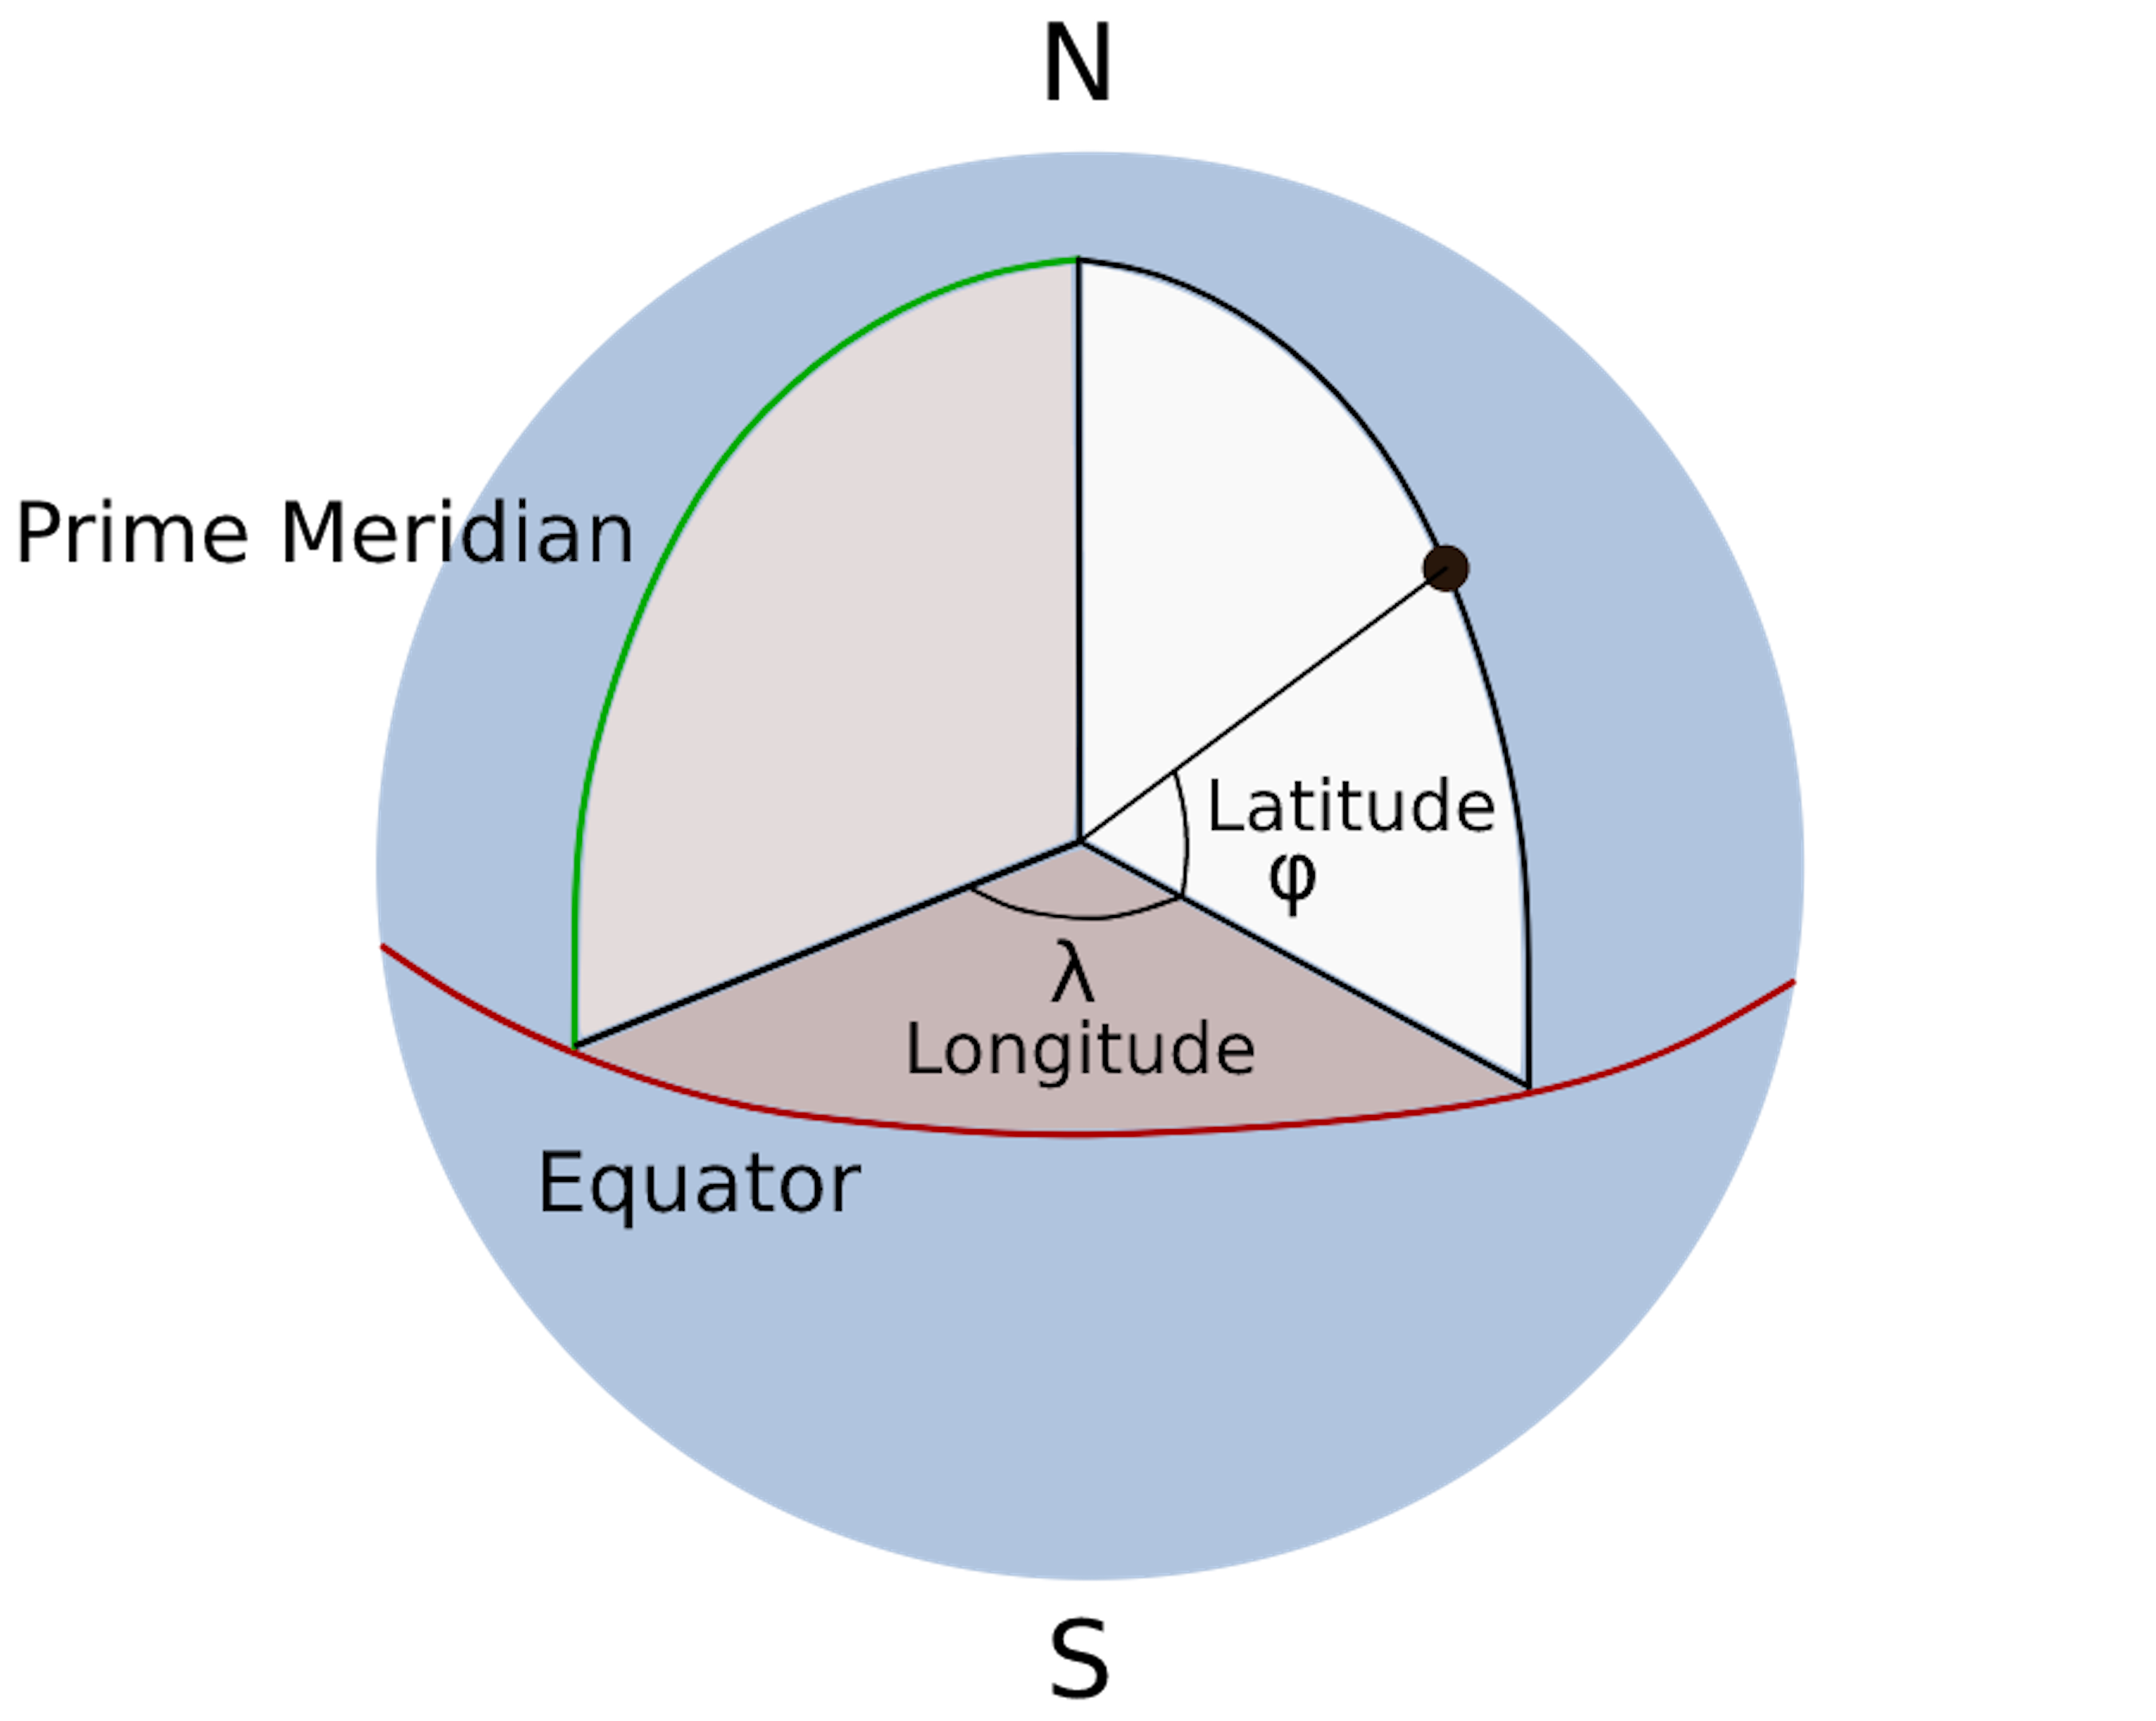
\includegraphics[width=0.9\textwidth]{latlong.png}
  \caption[Illustration of latitude and longitude]{Illustration of the earth, and how latitudes and longitudes are calculated with respect to the equator and the prime meridian.}
  \label{fig:latlong}
\end{figure}


Here are some examples on how to reference a source (where none is relevant to the text but just for illustration purposes only). One may cite a single reference by calling \cite{wolves_of_mount_mckinley}, or several in the same bracket by calling \cite{machine_learning, clustering_impossibility} when they are all related to the same statement. There are many different styles on how to cite, and how the layout and order of your citation style is presented. This is my favorite, as I find it neat and tidy \cite{sheep}. It will show up in order of appearance in the references section.
\cleardoublepage


\chapter{Methods}

Include the complete description of the methods used in your research here. \\

\noindent Below is an example of how subsectioning works. The sections and subsections will be included in the table of contents, while subsubsections will not be in the table of contents but still have their own title in the text.

\section{Section one}

\subsection{Subsection one}

\subsubsection{Subsubsection one}

\subsubsection{Subsubsection Two}

\subsection{Subsection Two}

\section{Section two}


\cleardoublepage


\chapter{Results}

\section{More figures}

This section includes some examples of different types of figures to include. A simple single figure is shown in figure \ref{fig:trajectory_angle}, while figure \ref{fig:cyclic} shows how three subfigures can be included together. Remember to change both the caption and the title in the square brackets before the caption, which will show up in the list of figures. \\

\noindent page fill page fill page fill page fill page fill page fill page fill page fill page fill page fill page fill page fill page fill page fill page fill page fill page fill page fill page fill page fill page fill page fill page fill page fill page fill page fill page fill page fill page fill page fill page fill page fill page fill page fill page fill page fill page fill page fill page fill page fill page fill page fill page fill page fill page fill page fill.

\begin{figure}[H]
  \centering
  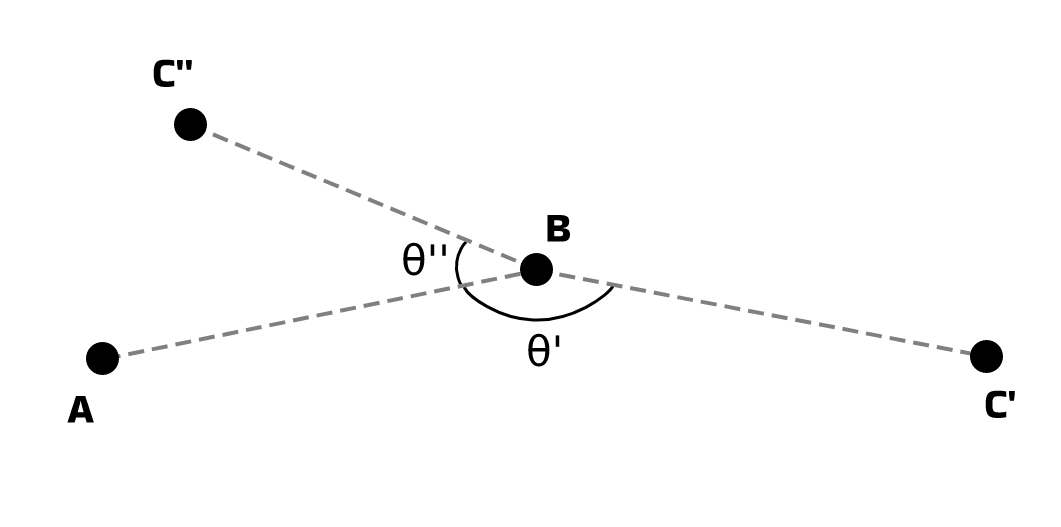
\includegraphics[width=1\textwidth]{Figures/trajectory angle.png}
  \caption[Trajectory angle]{The trajectory angle found for the trajectory ABC between the three points A, B and C. The two different C-points show the angle gotten for relatively unchanged directional trajectory with C', and opposite directional trajectory with C''.}
  \label{fig:trajectory_angle}
\end{figure}



\begin{figure}[H]
  \centering
  \subfloat[Time as a linear variable.]{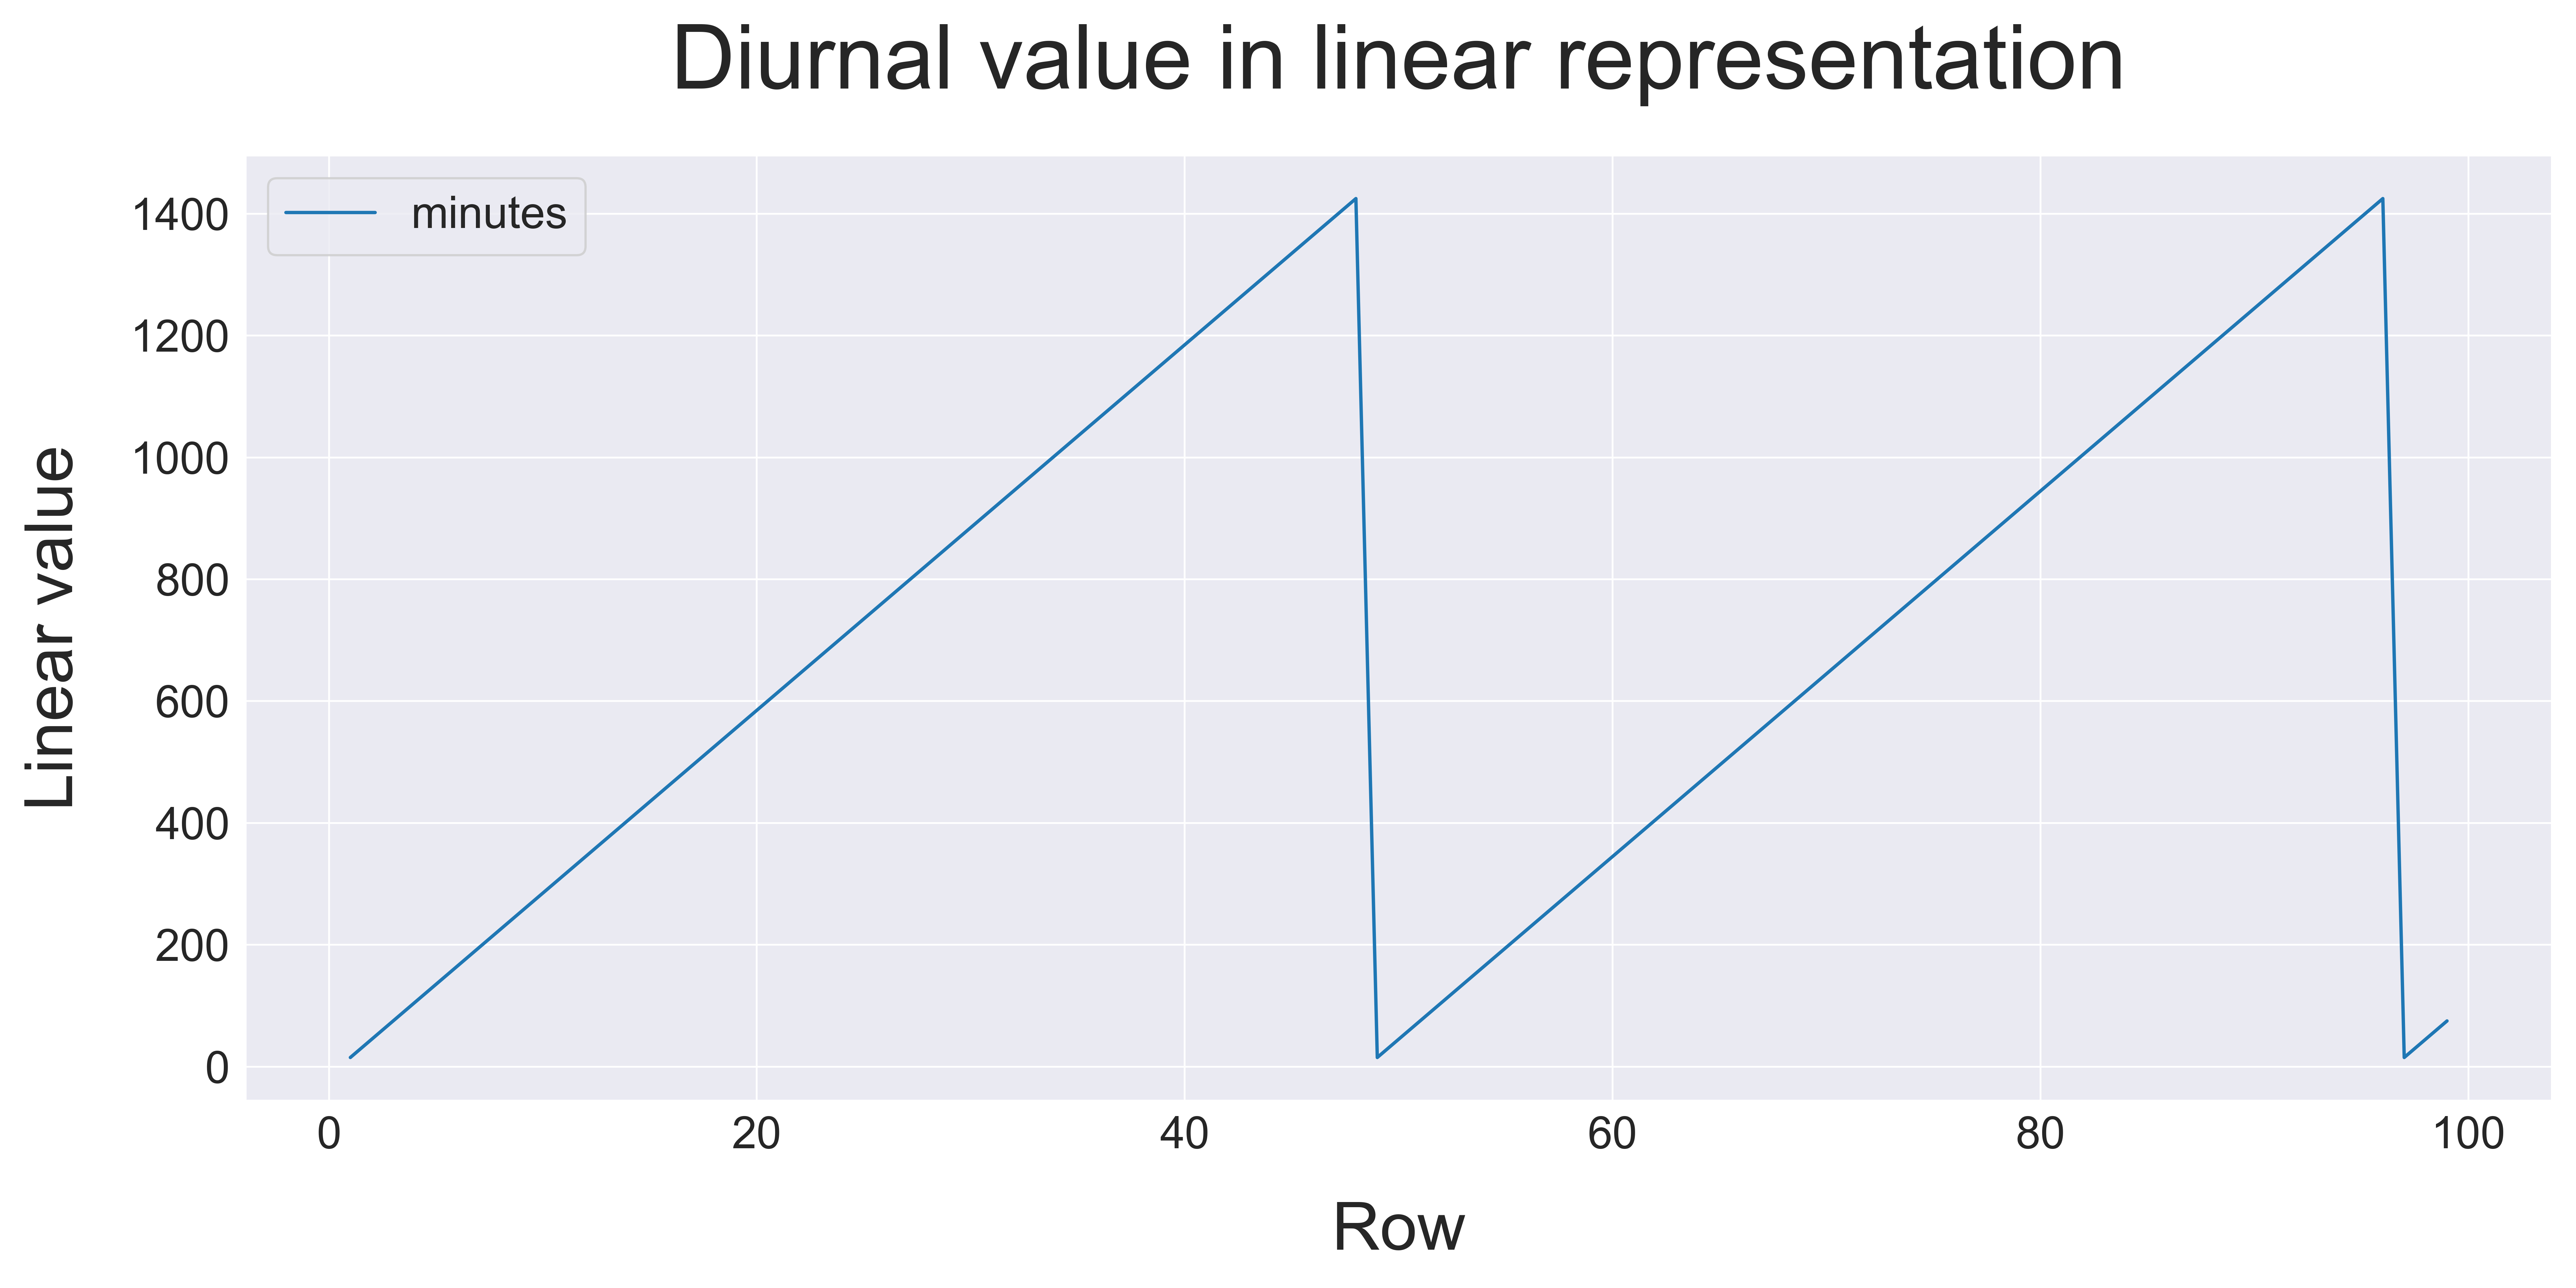
\includegraphics[width=0.75\textwidth]{Figures/diurnal_values_linear.png}\label{fig:diurnal_lin}}
  \hfill
  \subfloat[Time represented as pairs of sine and cosine.]{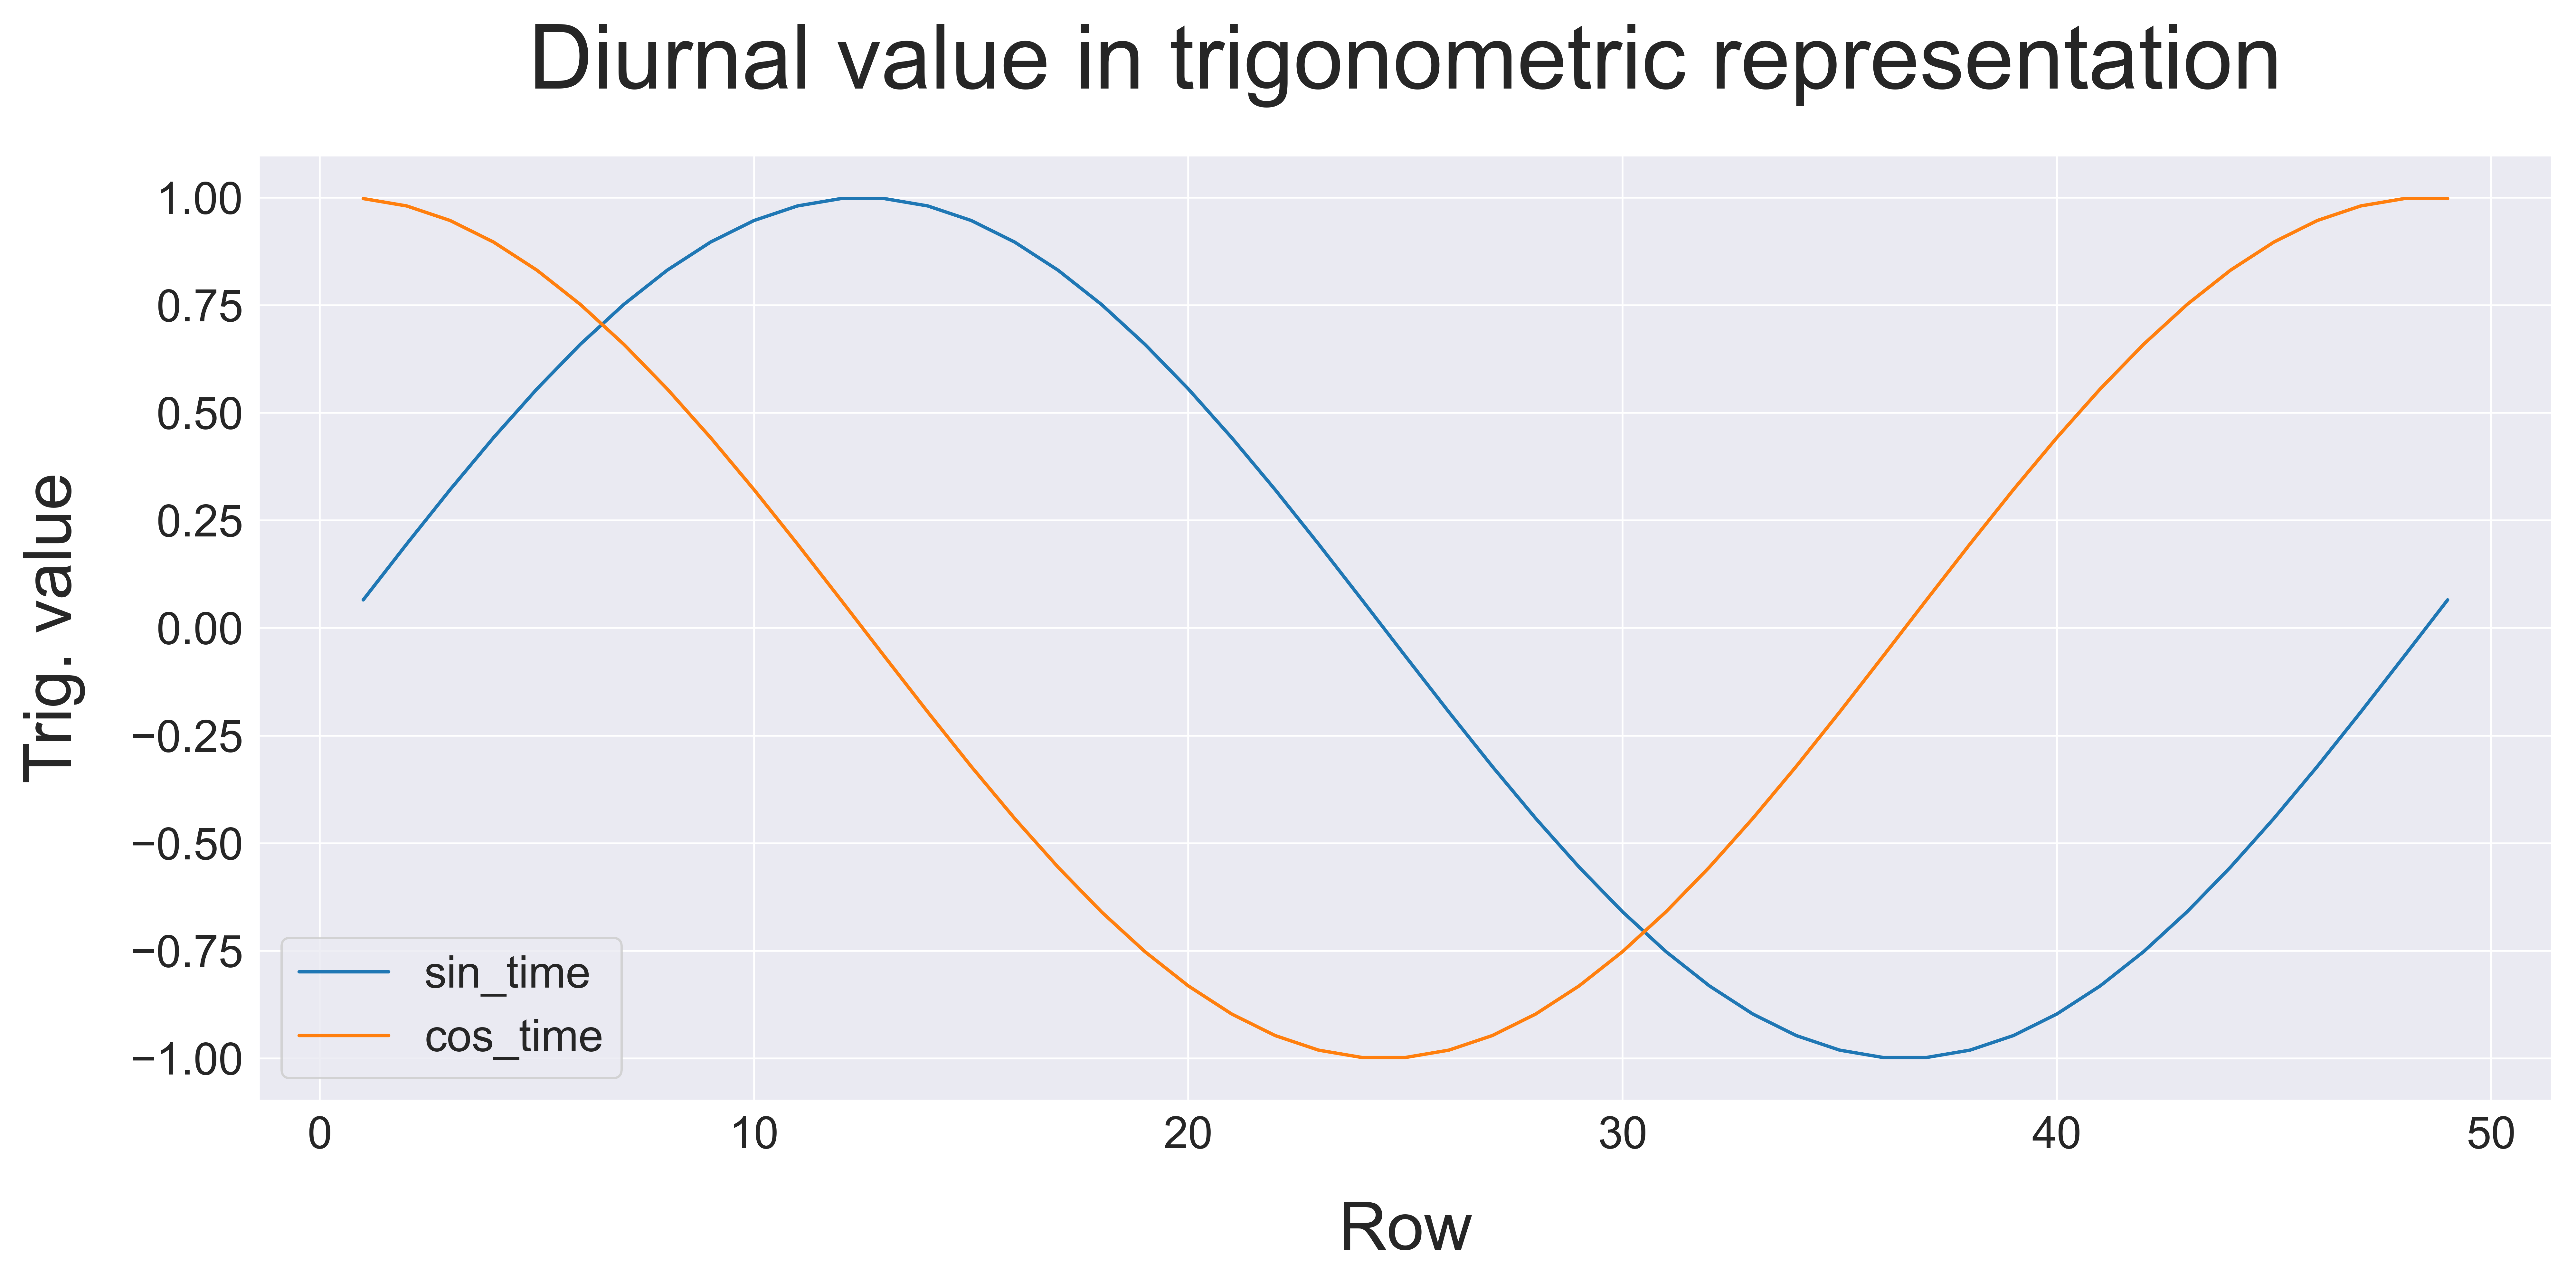
\includegraphics[width=0.75\textwidth]{Figures/diurnal_values_sine.png}\label{fig:diurnal_trig}}
  \hfill
  \subfloat[Time as a cyclic feature.]{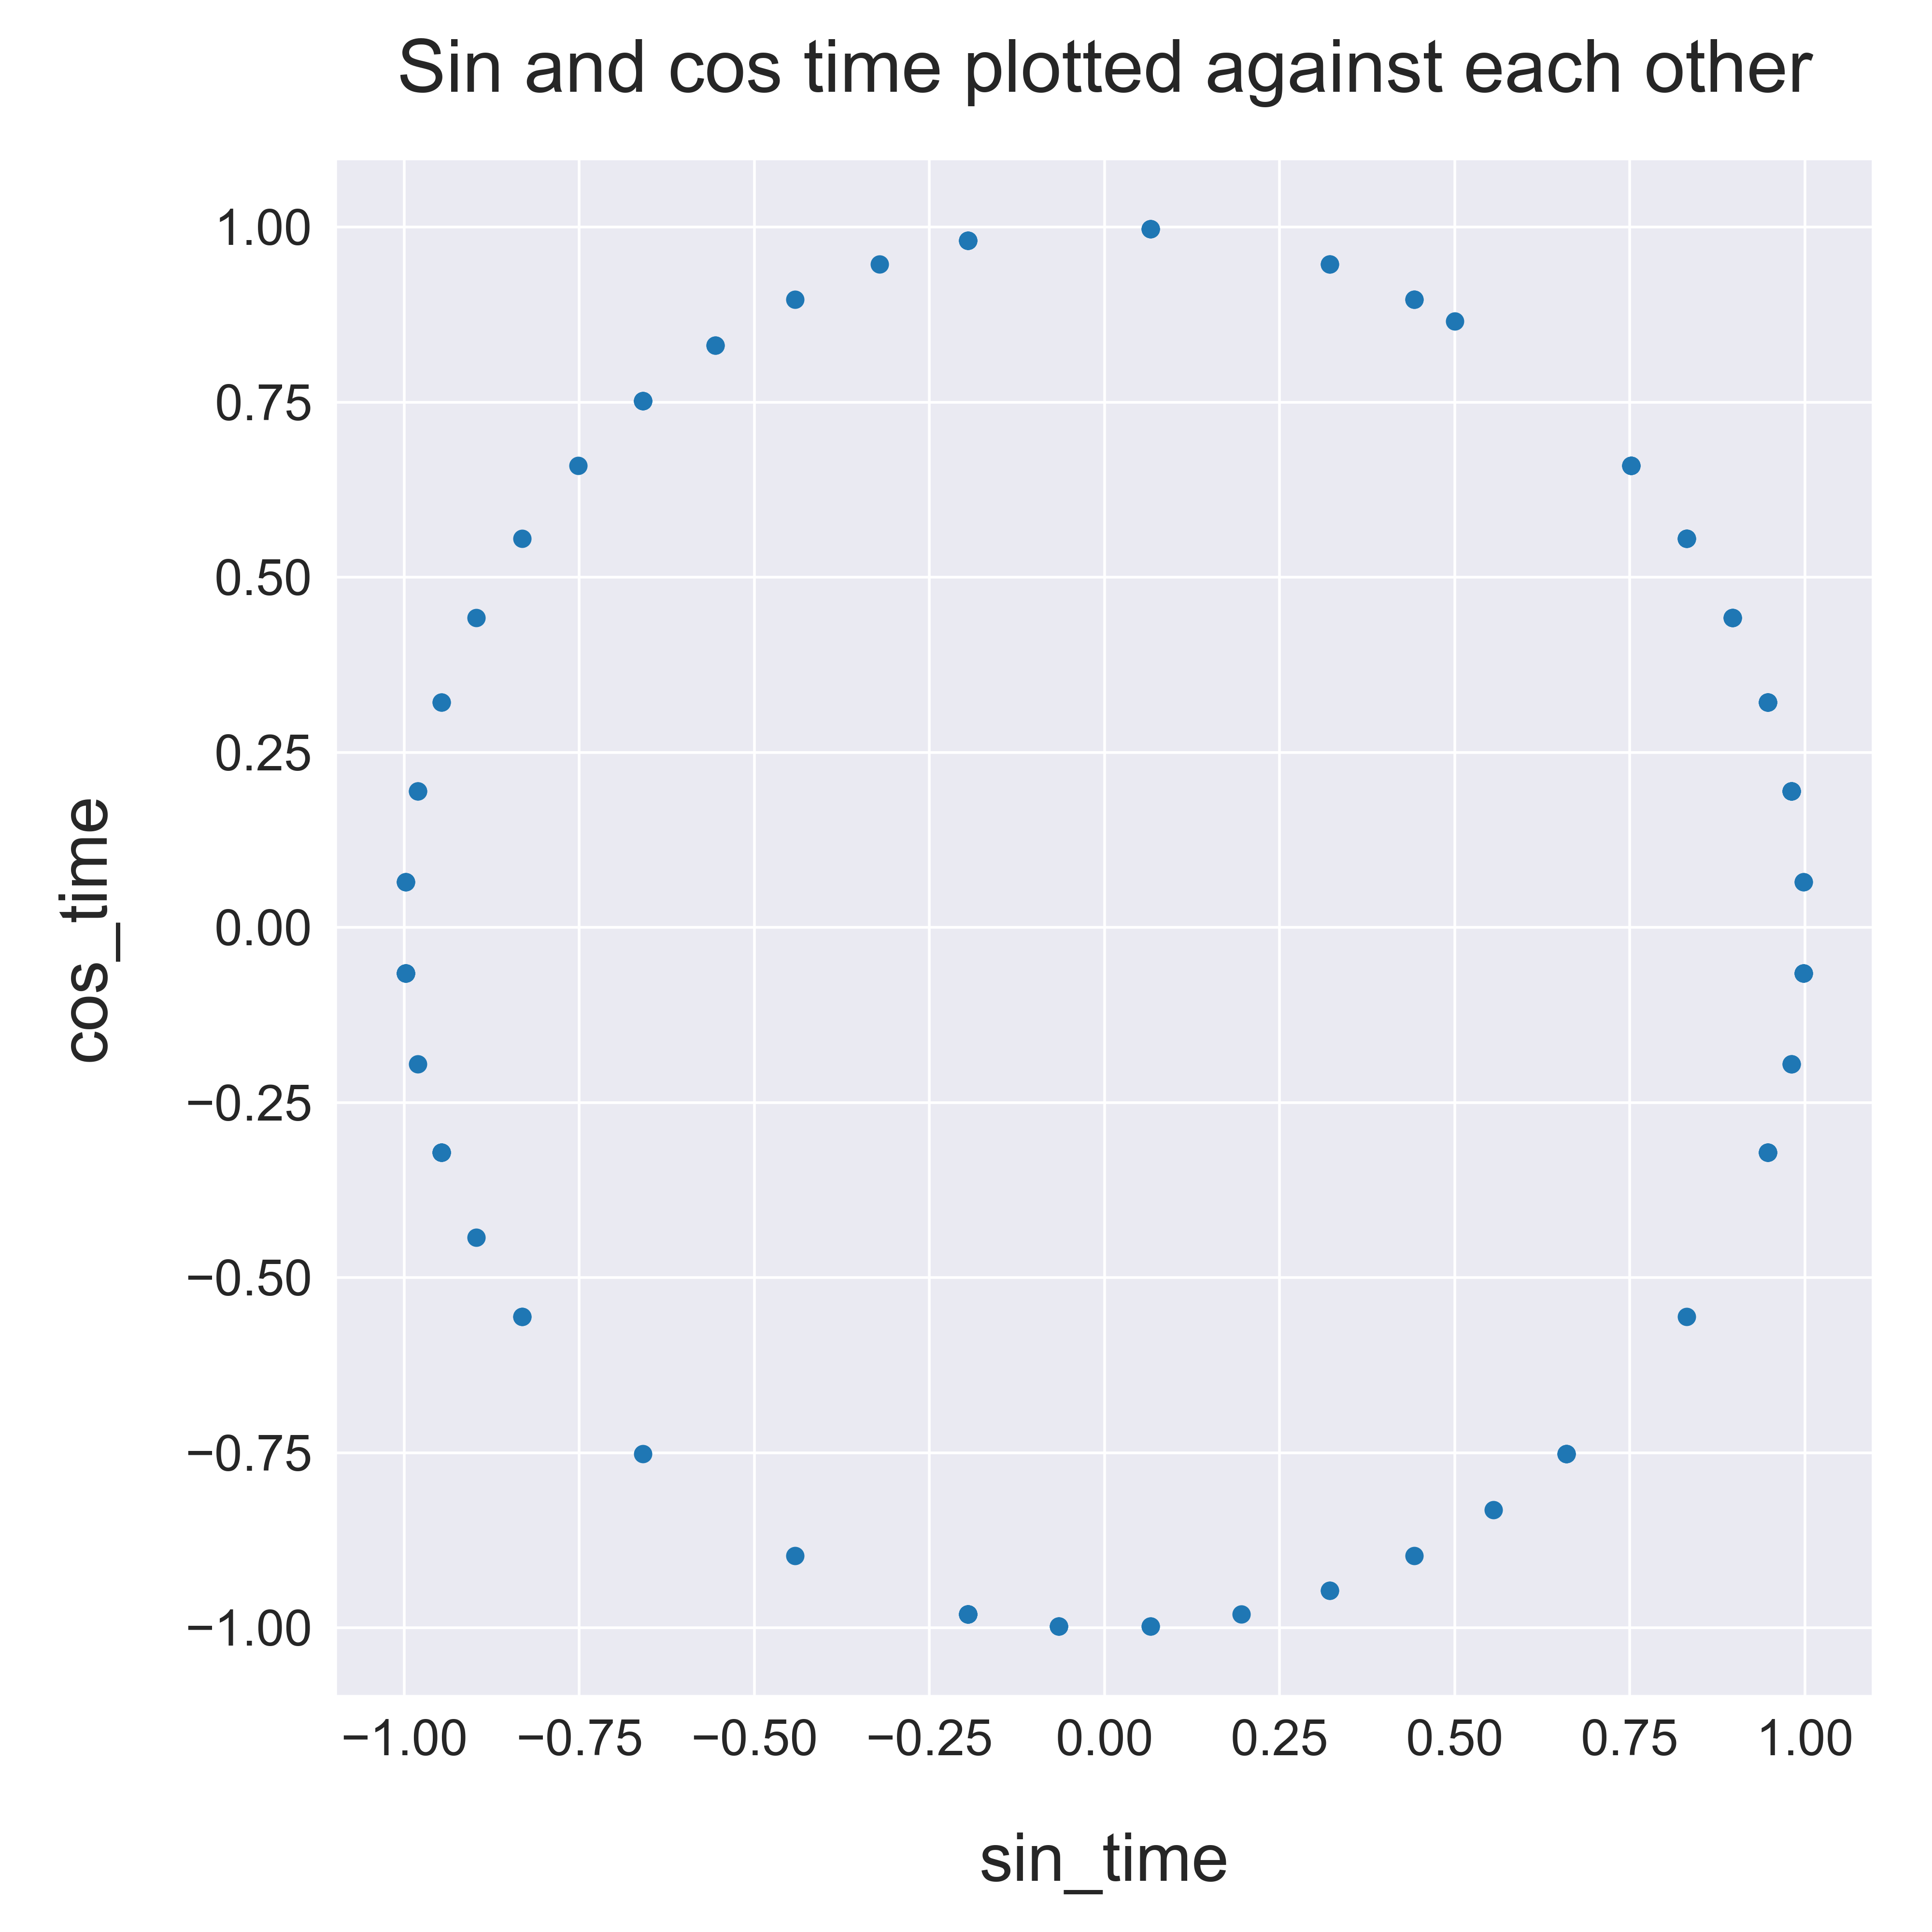
\includegraphics[width=0.6\textwidth]{Figures/diurnal_values_circle.png}\label{fig:diurnal_cyclic}}
  
  \caption[Time as a cyclic feature]{Figure (a) shows the time variable in the data for the first 100 rows using linear time as minutes past midnight, figure (b) shows the trigonometric time representation for one cycle where each time point has a unique sine and cosine-pair value, and figure (c) shows time as a cyclic feature with the trigonometric pairs.}
\label{fig:cyclic}
\end{figure}
\cleardoublepage


\chapter{Discussion}

Discuss your results here.

\section{Interpretation in terms of Black hole microstates}

\section{Future work}


Include a section about what should or could be done in future research, or explain any recommended next steps based on the results you got. This should be the last section in the discussion.
\cleardoublepage


\chapter{Conclusions}

Give a concise summary of your research and finding here, and include a short summary of any future work as well.
\cleardoublepage


\addcontentsline{toc}{chapter}{\protect\numberline{}References}
\printbibliography[title={References}] %you may change the title in the toc here if you want
\cleardoublepage


\chapter*{\LARGE \textbf{Appendices}}
\fancyhf{} %clear the header, it should be empty for the appendices
\renewcommand{\headrulewidth}{0pt} %no rule
\fancyfoot[C]{\thepage} %set the page numbers in the center of the footer instead 

%it is possible to set a different page numbering style for the appendix, but I personally just continued with the same page numbering as the main content as I find that more tidy
%\pagenumbering{roman}
%\setcounter{page}{1}
\addcontentsline{toc}{chapter}{\protect\numberline{}Appendices:}
\appendix
\chapter{Numerical Methods}
\label{app:numerical-methods}

The initial data of the BFSS system are $9$ $N \times N$ Hermitian matrices $X^{1}(0), \ldots, X^{K}(0)$ and their velocities $\dot{X}^{1}(0), \ldots, \dot{X}^{K}(0)$. Generating a random $N \times N$ Hermitian matrix is easy; generate $N^2$ random complex numbers using something like \texttt{RandomComplex} in Mathematica and assemble them into a complex $N \times N$ matrix $Z$ and take the Hermitian part $\frac{1}{2}(Z + Z^{\dagger})$.

The trace of the various matrices is unimportant because of "translation" symmetry $X^{k} \to X^{k} + \epsilon^{k} \boldsymbol{1}_N$ generated by the total momentum $\Tr \dot{X}^{k}$ which we set equal to zero, along with the center of mass position $\Tr X^{k}$, effectively working in the "center of mass" frame. We can thus remove traces of the various matrices above by $Z \to Z - \frac{\Tr Z}{N} \boldsymbol{1}_N $.

Of course, the problem with generating initial states like this is that they will generically be on completely disjoint phase trajectories. In order to study thermalization or some universal behavior, it is necessary to start with states of fixed macroscopic charges, which arise from the following symmetries.

\begin{enumerate}
  \item \textbf{Time translation} $\quad t \to t + \epsilon \quad \delta X^{k} = -\epsilon \dot{X}^{k}$
    \begin{equation}
      E = \Tr \left( \frac{1}{2} \dot{X}^{k} \dot{X}^{k} - \frac{1}{4} \comm{X^{i}}{X^{j}} \comm{X^{i}}{X^{j}} \right)
    \end{equation}
  \item \textbf{$\mathrm{SO}(K)$ Rotations} $\quad \omega_{k j} = -\omega_{j k} \quad \delta X^{k} = \omega_{k j} X^{j}$
    \begin{equation}
      J^{i j} = \Tr \left( X^{i} \dot{X}^{j} - X^{j} \dot{X}^{i} \right)
    \end{equation}
  \item \textbf{$\mathrm{SU}(N)$ Gauge transformations} $\quad M^{\dagger} = -M \quad \delta X^{k} = \comm{M}{X^{k}}$
    \begin{equation}
      G = \comm{X^{k}}{\dot{X}^{k}}
    \end{equation}
    To study the gauged system, $G$ must be set to zero.
\end{enumerate}

In total, there are $1 + \frac{K(K-1)}{2} + (N^2 - 1) + K = N^2 + \frac{K(K+1)}{2}$ real charges\footnote{The last term is the translation symmetry charge, the total momentum, which we set to zero}. 

The simplest way to fix the charges and satisfy the Gauge constraint is to set all the initial velocities to zero
\begin{equation}
  \dot{X}^i(0) = 0
\end{equation}
and we do exactly this.

It is very useful to rewrite the matrix variables in a convenient basis of the lie algebra $\mathfrak{su}(N)$ of $N \times N$ traceless Hermitian matrices. We use a generalized Gell-Mann type basis given by $\frac{N(N-1)}{2}$ real symmetric matrices, $\frac{N(N-1)}{2}$ imaginary antisymmetric matrices and $N-1$ real diagonal matrices (which also generate the Cartan subalgebra in this basis).
\begin{equation}\label{eqn:suN-basis}
  \begin{gathered}
    \underbrace{
      \frac{1}{2}\begin{pmatrix}
      & & & \\
      & & 1 & \\
      & 1 & & \\
      & & &
    \end{pmatrix}}_{\text{real symmetric}} \qquad%
    \underbrace{
      \frac{1}{2}\begin{pmatrix}
      & & & \\
      & & -i & \\
      & i & & \\
      & & &
    \end{pmatrix}}_{\text{imaginary antisymmetric}} \\
    \underbrace{
      \frac{1}{\sqrt{2r(r-1)}}\begin{pmatrix}
      1 & & & & \\
      & \ddots & & & \\
      & & 1 & & \\
      & & & 1-r & \\
      & & & &
    \end{pmatrix}}_{\text{real diagonal}}
  \end{gathered}
\end{equation}
These are normalized so that
\begin{equation}\label{eqn:cartan-killing}
\Tr t^{a} t^{b} = \frac{1}{2} \delta^{a b}
\end{equation}
We chose the physicist's convention for the Lie algebra of $\mathrm{SU}(N)$, meaning that the fundamental commutation relations of the $t^a$s contain a factor of $i$. They are
\begin{equation}
\comm{t^a}{t^b} = i f^{a b c} t^{c}
\end{equation}

It is easy to compute the structure constants $f^{a b c}$ in the basis we use \cref{eqn:suN-basis}. Due to the diagonal Cartan-Killing form \cref{eqn:cartan-killing}, the structure constants are completely antisymmetric in this basis. We can now expand all our matrix degrees of freedom in this basis
\begin{equation}
X^i(t) = x^{i}_{a}(t) t^a
\end{equation}
the matrix model equations of motion \cref{eqn:eom} can then be written as
\begin{equation}
\ddot{x}^i_a = f^{a e d} f^{e b c} x^i_b x^j_c x^j_d
\end{equation}

As stated in Chapter 3, the initial "positions" $x^i_a(0)$ are taken to be random. In particular, the procedure we follow to generate them is
\begin{enumerate}
  \item[a.] Generate $\tilde{X}^{i}_{a}$ as $K(N^2-1)$ random real numbers uniformly distributed in $(-1, 1)$.
  \item[b.] {
    Compute the energy $E$ of this state (with no velocity contribution) as%
    \begin{equation}
      E = \frac{1}{8} f^{a b e} f^{c d e} \tilde{X}^i_a \tilde{X}^j_b \tilde{X}^i_c \tilde{X}^j_d
    \end{equation}
  }
  \item[c.] {
    The random initial state we study $X^i_a$ is then given by
    \begin{equation}
      X^i_a = \lambda \tilde{X}^i_a \qquad \lambda = E^{-1/4}
    \end{equation}
  }
\end{enumerate}
By construction, the state just generated has energy $E = 1$. We now pose this as an initial value problem (IVP) 
\begin{align}
  \dot{x}^i_a &= p^i_a \qquad x^i_a(0) = X^i_a \\
  \dot{p}^i_a &= f^{a e d} f^{e b c} x^i_b x^j_c x^j_d \qquad p^i_a(0) = 0
\end{align}

Initial value problems (IVPs) are abundant in all of the sciences. There are numerous numerical methods and packages that can be used to solve IVPs of different types. The type of system we have, is, of course, a symplectic IVP since it is a Hamiltonian system. A standard numerical algorithm for solving symplectic systems is the Runge-Kutta-Nystroem family. We use the symplectic McLachlan symmetric B3A stepper implementing sixth order RKN \cite{doi:10.1137/0916010}. 

As a platform for our simulations, we chose to write C++ programs to optimize computational resources as much as possible. The Boost C++ library \cite{schälingboost} comes very handy in this regard as it already contains a robust implementation of symplectic RKN methods. Our simulation was run on the IITM Quantum cluster with parallel programming optimizations. An example of runtimes involved is: at $N = 9, K = 9$, and for a length of time $T = 1000$ and step size $dt = 0.1$, it takes around 5 hours on an Intel(R) Xeon(R) Gold 5220R CPU @ 2.20GHz on a single core.



\chapter{Gaussian Unitary Ensemble}
\label{app:gue}

Perhaps the simplest distribution for an $N \times N$ complex matrix $Y$ is one in which the real and imaginary parts of every matrix entry are distributed (independently and identically) according to a normal distribution. In particular, if
\begin{equation}
  Y = (y_{i j})_{i, j = 1}^{N}
\end{equation}
then the distribution would be
\begin{equation}\label{eqn:complex-mat-dist}
  \begin{aligned}
    p(y_{i j}) &= \prod_{i j} \frac{1}{2\pi \sigma^2} \exp \left( -\frac{1}{2 \sigma^2} y_{i j} \overline{y}_{i j} \right) \\
    &= \left( \frac{1}{2\pi \sigma^2} \right)^{N^2} \exp \left( -\frac{1}{2 \sigma^2} \sum_{i j} y_{i j} \overline{y}_{i j} \right) \\
    &= \frac{1}{Z} \exp \left( -\frac{1}{2 \sigma^2} \Tr Y^\dagger Y \right)
  \end{aligned}
\end{equation}
with
\begin{equation}
  \log Z = N^2 \log(2 \pi \sigma^2)
\end{equation}
being the partition function used for normalization.

However, we are interested in traceless Hermitian matrices. But once one can generate random "normal" complex matrices $Y$, it is elementary to transform them into traceless Hermitian matrices. We do this in two steps
\begin{enumerate}
  \item[a.] {
    Pick out the Hermitian part $\tilde{X}$
    \begin{equation}
      Y \to \tilde{X} = \frac{Y + Y^{\dagger}}{2}
    \end{equation}
  }
  \item[b.] {
    Remove the trace
    \begin{equation}
      \tilde{X} \to X = \tilde{X} - \frac{Tr\tilde{X}}{N} \mathbf{1}_N
    \end{equation}
  }
\end{enumerate}

The distribution of the random matrix variable $\tilde{X}$ has a distribution closely related to \cref{eqn:complex-mat-dist}, namely
\begin{equation}
  p(\tilde{X}) = \frac{1}{Z_{\mathrm{GUE}}} \exp \left( -\frac{1}{2 \sigma^2} \Tr \tilde{X}^2 \right)
\end{equation}
This is called the Gaussian Unitary Ensemble (GUE). Although the functional form of the distribution looks very much like \cref{eqn:complex-mat-dist}, the partition function $Z_{\mathrm{GUE}}$ has changed since the probability measure now contains only half as many integration variables as before ($N^2$ now, $2N^2$ for $Y$).

Finally, removing the trace results in the so-called traceless GUE with, again, the same functional form for the distribution but a different partition function we call $Z_\mathrm{tGUE}$.

It is interesting to look at the distribution of eigenvalues $\left( \lambda_1, \ldots, \lambda_N \right)$ resulting from, say, GUE. The joint distribution (for the case $\sigma = 1$) turns out to be
\begin{equation}
  \rho(\lambda_1, \ldots, \lambda_N) = \frac{1}{\mathcal{Z}} e^{-\frac{1}{2} \sum_{i = 1}^{N} \lambda_i^2} \prod_{i < j} (\lambda_i - \lambda_j)^2
\end{equation}
where $\mathcal{Z}$ is given by a kind of Mehta's integral
\begin{equation}
  \mathcal{Z} = (2 \pi)^{N/2} \prod_{k = 1}^{N} k!
\end{equation}

One can integrate out all but one of the eigenvalues to obtain the marginal distribution of one of the eigenvalues. It can be shown that it is the same distribution as what one would obtain if one were to combine all the eigenvalues and treat them independently (even though they are not independent). Incidentally, the non-independence of the eigenvalues results in physical phenomena where a random matrix description works, such as level repulsion. After a little bit of work and using the machinery of orthogonal polynomials, this results in
\begin{equation}
  \rho_{\mathrm{GUE}}(\lambda) = \frac{1}{N \sqrt{2\pi}} e^{-\lambda^2/2} \sum_{k = 0}^{N-1} \frac{1}{2^k k!} H_k\left(\frac{\lambda}{\sqrt{2}}\right)^2
\end{equation}
where $H_k$ denotes the $k^\mathrm{th}$ Hermite polynomial. Further, the asymptotic formulae for the Hermite polynomials can be used to prove the Wigner semicircle law (that holds as $N \to \infty$).

The corresponding formulae for traceless GUE can also be obtained with some work, but as of now, we do not have a closed-form distribution of eigenvalues. It is, however, interesting to note a relationship between the eigenvalue distribution of GUE and traceless GUE (see, e.g., \cite{1999math......4042T}) that schematically looks like
\begin{equation}
  \rho_{\mathrm{GUE}}(\lambda) = \sqrt{\frac{N}{\pi}} \int_{\mathbb{R}} \text{d} t e^{-N t^2} \rho_{\mathrm{tGUE}}(\lambda - t)
\end{equation}

For an accessible introduction to the theory of random matrices, see \cite{Livan_2018}. 



\chapter{Matrix Spherical Harmonics}
\label{app:matrix-harmonics}

In trying to understand a theory of matrices, it is useful to think of a configuration of them (traceless, Hermitian, in our case) as functions on $\B{S}^2$. In particular, these functions can be restricted to square integrable $L^2(\B{S}^2)$. Another way to approach this is by considering the matrices as a truncation of the set of all square-integrable functions on $\B{S}^2$. Thus, one has a map $\mu$.
  \begin{align}
    \mu \colon \mathfrak{u}(N) &\to L^2(\B{S}^2) \cr
    X &\mapsto \mu(X)
  \end{align}
  This map must respect the Hilbert space structure on the two sides. In addition, the two sides have a natural action of $\mathrm{SU}(2)$ defined on them. We can require our map to be equivariant with respect to this action. In total, we can list three requirements for $\mu$
  \begin{enumerate}
    \item Linearity
      \begin{equation}
        \mu(\alpha X + \beta Y) \; = \; \alpha \, \mu(X) + \beta \, \mu(Y)
      \end{equation}
    \item Preserve inner product
      \begin{equation}
        \underbrace{\frac{1}{N} \Tr X^\dagger Y}_{\substack{\text{Hilbert-Schmidt inner} \\ \text{product on }\mathfrak{u}(N)}} \; = \; \underbrace{\int_{\B{S}^2} \text{d}\Omega \, \mu(X)^* \mu(Y)}_{L^2\text{ inner product}}
      \end{equation}
    \item Preserve the action of $\mathrm{SU}(2)$\\
      $\mathrm{SU}(2)$ acts on $\mathfrak{u}(N)$ by it's adjoint action. On $\B{S}^2$, $\mathrm{SU}(2)$ acts by rotation which is pushed over to $L^2(\B{S}^2)$
      \begin{align}
        \mathfrak{u}(N) \ni X \; &\xrightarrow{U \, \in \, \mathrm{SU}(2)} \; U^\dagger X U \cr
        L^2(\B{S}^2) \ni f(\theta, \phi) \; &\xrightarrow{U \, \in \, \mathrm{SU}(2)} \; f(U^{-1} (\theta, \phi)) \cr
        U^\dagger X U \; &\xrightarrow{\quad\mu\quad} \; \mu(X)(U^{-1} (\theta, \phi))
      \end{align}
      Or, at the level of $\mathrm{SU}(2)$ generators $\mathfrak{g} = \alpha_i J^i$
      \begin{equation}
        \comm{J^i}{X} \; \xrightarrow{\quad\mu\quad} \; \xi^{(i)}(\mu(X))
      \end{equation}
      where $\xi^{(i)}$ are the Killing fields associated to $J^i$. Explicitly,
      \begin{equation}
        \xi^{(i)} = -i \epsilon_{i j k} x^j \frac{\partial}{\partial x^k} \quad \text{with} \quad x^k = (\sin \theta \cos \phi, \sin \theta \sin \phi, \cos \theta)
      \end{equation}
  \end{enumerate}

  To explicitly construct such a map, it is enough to define it on a basis $\{\B{Z}_a\}$ of $\mathfrak{u}(N)$. However, we would also like to make use of the rotational covariance, which is more manifest on the right-hand side of this map: We know that spherical harmonics $Y^{j}_{m}$ ($j = 0, 1, \ldots$ and $m = -j, -j+1, \ldots, j$) give a convenient orthonormal basis of $L^2(\B{S}^2)$ which also transforms nicely under $\mathfrak{su}(2)$. That is, every $j$-multiplet of $Y^{j}_{m}$ furnishes the usual spin-$j$ representation of $\mathfrak{su}(2)$. For example,
  \begin{align}
    \xi^{3}Y^{j}_{m} &= m Y^{j}_{m} \cr
    \xi^{i} \xi^{i} Y^{j}_{m} &= j(j+1) Y^{j}_{m} \cr
    \frac{1}{4\pi} \int_{\B{S}^2} \text{d}\Omega \, {Y^{j_1}_{m_1}}^* {Y^{j_2}_{m_2}} &= \delta^{j_1}_{j_2} \delta^{m_1}_{m_2} 
  \end{align}

  Thus, if we can define the inverse map $\mu^{-1}$ on these $Y^{j}_{m}$, we'd be done. It is clear, though, that the map $\mu$ as it is defined above fails to be surjective: $L^2(\B{S}^2)$ is an infinite dimensional vector space whereas $\mathfrak{u}(N)$ is $N^2$ dimensional. However, we can still define $\mu$ on a truncated set of $Y^{j}_{m}$. The truncation is easy to derive: each $j$-multiplet is $(2j+1)$ dimensional. Suppose we truncate at $j = j_{\text{max}}$: i.e., we only take $j \in \{0, 1, \ldots, j_{\text{max}}\}$, then it must be that
  \begin{equation}
    \sum_{j=0}^{j_{\text{max}}} (2j+1) = (j_{\text{max}}+1)^2 = N^2 \quad \implies \quad j_{\text{max}} = N-1
  \end{equation}
  Therefore, we must define the so-called \textit{matrix harmonics} $Z^{j}_{m} \coloneqq \mu^{-1}(Y^j_m)$ ($j = 0, 1, \ldots, N-1$ and $m = -j, -j+1, \ldots, j$)\\

  Fortunately, we do have some special $\mathfrak{u}(N)$ matrices that can help: the spin-$\frac{N-1}{2}$ dimensional representation of $\mathfrak{su}(2)$. For the spin-$j$ irrep
  \begin{equation}
    J^{3}_{s s'} \coloneqq \mel{j\,s'}{J^3}{j\,s} = s \, \delta_{s s'}
  \end{equation}
  And $J^{1}$, $J^2$ are given in terms of $J^{\pm} \coloneqq J^1 \pm i J^2$
  \begin{align}
    J^\pm_{s s'} &= C^{\pm}_{j s} \, \delta_{s \pm 1, s'} \cr
    C^{\pm}_{j s} &= \sqrt{(j \mp s)(j \pm s + 1)}
  \end{align}
  The $Z^j_m$ can be found by starting at the lowest "rung of the ladder," $Z^j_{-j}$ and successively applying $J^+$
  \begin{equation}
    Z^j_m = \frac{1}{C^{+}_{j \, m-1}} \comm{J^+}{Z^j_{m-1}}
  \end{equation}
  Note that $\comm{J^-}{Z^j_{-j}} = 0$ so a plausible choice could be $Z^j_{-j} = f(J^-)$. Also, $\comm{J^+}{{(J^-)}^m} \sim {(J^-)}^{m-1}$, so we take
  \begin{equation}
    Z^j_{-j} = c \, {(J^-)}^{j}
  \end{equation}
  where $c$ is found by requiring orthonormality
  \begin{equation}
    \frac{1}{N} \Tr ({Z^{j_1}_{m_1}})^{\dagger} Z^{j_2}_{m_2} = \delta^{j_1}_{j_2} \delta^{m_1}_{m_2}
  \end{equation}


\end{document}
